\documentclass{article}
\usepackage{pgfplots}
\usepackage{color}
\usepackage{xcolor}
\pgfplotsset{compat=1.15}
\usepackage{amsmath}
\usepackage{amssymb}

\begin{document}

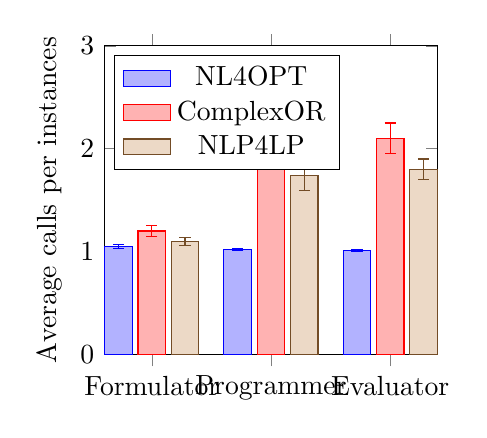
\begin{tikzpicture}
\begin{axis}[
    ybar, area legend,
    enlarge x limits=0.2, 
    legend style={
      anchor=north,
      legend image code/.code={ % Add this part
        \draw[##1,/tikz/.cd,yshift=-0.25em]
        (0cm,0cm) rectangle (3pt,0.8em);},
    },
    legend pos=north west,
    ylabel={Average calls per instances},
    symbolic x coords={Formulator, Programmer, Evaluator},
    xtick=data,
    ymin=0, ymax=3,
    height=5.5cm,
    width=0.48\textwidth,
    error bars/y dir=both,
    error bars/y explicit,
    ]

\addplot+[
    error bars/.cd,
    y dir=both,
    y explicit,
] coordinates {
    (Formulator,1.05) +- (0,0.02)
    (Programmer,1.02) +- (0,0.01)
    (Evaluator,1.01) +- (0,0.01)};
\addlegendentry{NL4OPT}

\addplot+[
    error bars/.cd,
    y dir=both,
    y explicit,
] coordinates {
    (Formulator,1.2) +- (0,0.05)
    (Programmer,2.0) +- (0,0.2)
    (Evaluator,2.1) +- (0,0.15)};
\addlegendentry{ComplexOR}

\addplot+[
    error bars/.cd,
    y dir=both,
    y explicit,
] coordinates {
    (Formulator, 1.1) +- (0,0.04)
    (Programmer, 1.74) +- (0,0.15)
    (Evaluator, 1.8) +- (0,0.1)};
\addlegendentry{NLP4LP}

\end{axis}
\end{tikzpicture}

\end{document}